\section{Stato dell'arte}
\subsection{Firme Digitali}
Una firma digitale è uno schema matematico per dimostrare l'autenticità di un messaggio, o in generale, di un documento. Di fatto, permette di verificare che il documento non sia stato modificato dopo la creazione, da terze parti illecite.
Si utilizzano algoritmi di cifratura con chiave pubblica. L'idea è di firmare, ovverro codificare con la propria chiave privata, un hash del documento ed appenderlo
\subsection{Face Recognition}
stato arte face recognition
\subsection{QR Code}
Si tratta di un codice a barre bidimensionale
a matrice, composto da moduli neri disposti all'interno di uno schema di forma quadrata. 
Viene impiegato per memorizzare informazioni generalmente destinate ad essere lette 
tramite un dispositivo mobile ( es. smartphone, tablet ).
\begin{flushright}
\begin{figure}[htbp]
   \centering
   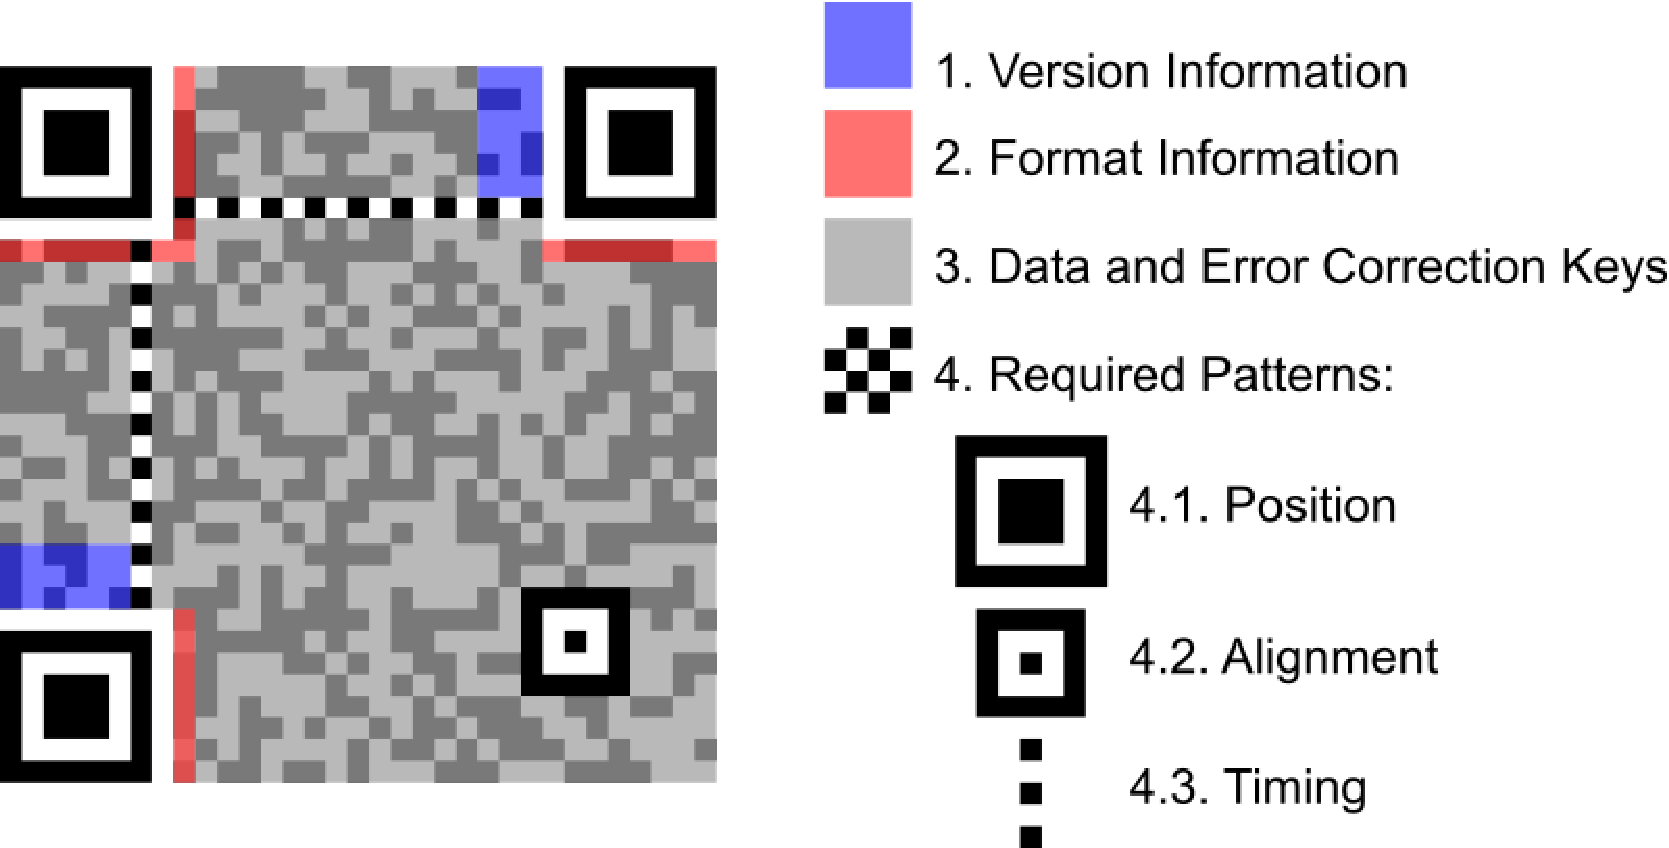
\includegraphics[width=4cm]{img/qrcodestruct}
   \caption{Struttura Qrcode\label{qrgen}}
\end{figure}
\end{flushright}
Un solo crittogramma può contenere fino a 7.089 caratteri numerici o 4.296 alfanumerici.
Il loro utilizzo è per lo più
\begin{center}
\begin{tabular}{|c|}
\hline\textbf{ Capacità di memorizzazione} \\ 
\hline Solo numerico: max 7.089 caratteri. \\ 
\hline Alfanumerico: max 4.296 caratteri  \\ 
\hline  Binario (8 bit): max 2.953 byte \\ 
\hline Kanji/Kana: max 1.817 caratteri.\\
\hline 
\end{tabular} 
\linebreak 
\linebreak
\linebreak 
\linebreak
\begin{tabular}{|c|}
\hline\textbf{Capacità di correzione degli errori} \\ 
\hline  Livello L: circa il 7\%  delle parole in codice può essere ripristinato. \\ 
\hline  Livello M: circa il 15\% delle parole può essere ripristinato \\ 
\hline  Livello Q: circa il 25\% delle parole può essere ripristinato\\ 
\hline  Livello H: circa il 30\%  delle parole può essere ripristinato\\
\hline 
\end{tabular} 
\end{center}